% Options for packages loaded elsewhere
\PassOptionsToPackage{unicode}{hyperref}
\PassOptionsToPackage{hyphens}{url}
%
\documentclass[
  11 pt,
]{article}
\usepackage{amsmath,amssymb}
\usepackage{lmodern}
\usepackage{ifxetex,ifluatex}
\ifnum 0\ifxetex 1\fi\ifluatex 1\fi=0 % if pdftex
  \usepackage[T1]{fontenc}
  \usepackage[utf8]{inputenc}
  \usepackage{textcomp} % provide euro and other symbols
\else % if luatex or xetex
  \usepackage{unicode-math}
  \defaultfontfeatures{Scale=MatchLowercase}
  \defaultfontfeatures[\rmfamily]{Ligatures=TeX,Scale=1}
\fi
% Use upquote if available, for straight quotes in verbatim environments
\IfFileExists{upquote.sty}{\usepackage{upquote}}{}
\IfFileExists{microtype.sty}{% use microtype if available
  \usepackage[]{microtype}
  \UseMicrotypeSet[protrusion]{basicmath} % disable protrusion for tt fonts
}{}
\makeatletter
\@ifundefined{KOMAClassName}{% if non-KOMA class
  \IfFileExists{parskip.sty}{%
    \usepackage{parskip}
  }{% else
    \setlength{\parindent}{0pt}
    \setlength{\parskip}{6pt plus 2pt minus 1pt}}
}{% if KOMA class
  \KOMAoptions{parskip=half}}
\makeatother
\usepackage{xcolor}
\IfFileExists{xurl.sty}{\usepackage{xurl}}{} % add URL line breaks if available
\IfFileExists{bookmark.sty}{\usepackage{bookmark}}{\usepackage{hyperref}}
\hypersetup{
  pdftitle={Final Report},
  pdfauthor={Grace Lee and Jiyun Hyo},
  hidelinks,
  pdfcreator={LaTeX via pandoc}}
\urlstyle{same} % disable monospaced font for URLs
\usepackage[margin=1in]{geometry}
\usepackage{color}
\usepackage{fancyvrb}
\newcommand{\VerbBar}{|}
\newcommand{\VERB}{\Verb[commandchars=\\\{\}]}
\DefineVerbatimEnvironment{Highlighting}{Verbatim}{commandchars=\\\{\}}
% Add ',fontsize=\small' for more characters per line
\usepackage{framed}
\definecolor{shadecolor}{RGB}{248,248,248}
\newenvironment{Shaded}{\begin{snugshade}}{\end{snugshade}}
\newcommand{\AlertTok}[1]{\textcolor[rgb]{0.94,0.16,0.16}{#1}}
\newcommand{\AnnotationTok}[1]{\textcolor[rgb]{0.56,0.35,0.01}{\textbf{\textit{#1}}}}
\newcommand{\AttributeTok}[1]{\textcolor[rgb]{0.77,0.63,0.00}{#1}}
\newcommand{\BaseNTok}[1]{\textcolor[rgb]{0.00,0.00,0.81}{#1}}
\newcommand{\BuiltInTok}[1]{#1}
\newcommand{\CharTok}[1]{\textcolor[rgb]{0.31,0.60,0.02}{#1}}
\newcommand{\CommentTok}[1]{\textcolor[rgb]{0.56,0.35,0.01}{\textit{#1}}}
\newcommand{\CommentVarTok}[1]{\textcolor[rgb]{0.56,0.35,0.01}{\textbf{\textit{#1}}}}
\newcommand{\ConstantTok}[1]{\textcolor[rgb]{0.00,0.00,0.00}{#1}}
\newcommand{\ControlFlowTok}[1]{\textcolor[rgb]{0.13,0.29,0.53}{\textbf{#1}}}
\newcommand{\DataTypeTok}[1]{\textcolor[rgb]{0.13,0.29,0.53}{#1}}
\newcommand{\DecValTok}[1]{\textcolor[rgb]{0.00,0.00,0.81}{#1}}
\newcommand{\DocumentationTok}[1]{\textcolor[rgb]{0.56,0.35,0.01}{\textbf{\textit{#1}}}}
\newcommand{\ErrorTok}[1]{\textcolor[rgb]{0.64,0.00,0.00}{\textbf{#1}}}
\newcommand{\ExtensionTok}[1]{#1}
\newcommand{\FloatTok}[1]{\textcolor[rgb]{0.00,0.00,0.81}{#1}}
\newcommand{\FunctionTok}[1]{\textcolor[rgb]{0.00,0.00,0.00}{#1}}
\newcommand{\ImportTok}[1]{#1}
\newcommand{\InformationTok}[1]{\textcolor[rgb]{0.56,0.35,0.01}{\textbf{\textit{#1}}}}
\newcommand{\KeywordTok}[1]{\textcolor[rgb]{0.13,0.29,0.53}{\textbf{#1}}}
\newcommand{\NormalTok}[1]{#1}
\newcommand{\OperatorTok}[1]{\textcolor[rgb]{0.81,0.36,0.00}{\textbf{#1}}}
\newcommand{\OtherTok}[1]{\textcolor[rgb]{0.56,0.35,0.01}{#1}}
\newcommand{\PreprocessorTok}[1]{\textcolor[rgb]{0.56,0.35,0.01}{\textit{#1}}}
\newcommand{\RegionMarkerTok}[1]{#1}
\newcommand{\SpecialCharTok}[1]{\textcolor[rgb]{0.00,0.00,0.00}{#1}}
\newcommand{\SpecialStringTok}[1]{\textcolor[rgb]{0.31,0.60,0.02}{#1}}
\newcommand{\StringTok}[1]{\textcolor[rgb]{0.31,0.60,0.02}{#1}}
\newcommand{\VariableTok}[1]{\textcolor[rgb]{0.00,0.00,0.00}{#1}}
\newcommand{\VerbatimStringTok}[1]{\textcolor[rgb]{0.31,0.60,0.02}{#1}}
\newcommand{\WarningTok}[1]{\textcolor[rgb]{0.56,0.35,0.01}{\textbf{\textit{#1}}}}
\usepackage{graphicx}
\makeatletter
\def\maxwidth{\ifdim\Gin@nat@width>\linewidth\linewidth\else\Gin@nat@width\fi}
\def\maxheight{\ifdim\Gin@nat@height>\textheight\textheight\else\Gin@nat@height\fi}
\makeatother
% Scale images if necessary, so that they will not overflow the page
% margins by default, and it is still possible to overwrite the defaults
% using explicit options in \includegraphics[width, height, ...]{}
\setkeys{Gin}{width=\maxwidth,height=\maxheight,keepaspectratio}
% Set default figure placement to htbp
\makeatletter
\def\fps@figure{htbp}
\makeatother
\setlength{\emergencystretch}{3em} % prevent overfull lines
\providecommand{\tightlist}{%
  \setlength{\itemsep}{0pt}\setlength{\parskip}{0pt}}
\setcounter{secnumdepth}{-\maxdimen} % remove section numbering
\ifluatex
  \usepackage{selnolig}  % disable illegal ligatures
\fi

\title{Final Report}
\usepackage{etoolbox}
\makeatletter
\providecommand{\subtitle}[1]{% add subtitle to \maketitle
  \apptocmd{\@title}{\par {\large #1 \par}}{}{}
}
\makeatother
\subtitle{due November 16, 2021 by 11:59 PM}
\author{Grace Lee and Jiyun Hyo}
\date{November 16, 2021}

\begin{document}
\maketitle

\hypertarget{load-packages}{%
\section{Load Packages}\label{load-packages}}

\begin{Shaded}
\begin{Highlighting}[]
\FunctionTok{library}\NormalTok{(dplyr)}
\FunctionTok{library}\NormalTok{(tidyverse)}
\FunctionTok{library}\NormalTok{(sf)}
\FunctionTok{library}\NormalTok{(viridis)}
\FunctionTok{library}\NormalTok{(tidyverse)}
\FunctionTok{library}\NormalTok{(tidymodels)}
\FunctionTok{library}\NormalTok{(ggspatial) }\CommentTok{\#for scale annotation}
\FunctionTok{library}\NormalTok{(ggplot2)}
\end{Highlighting}
\end{Shaded}

\hypertarget{load-data}{%
\section{Load Data}\label{load-data}}

\begin{Shaded}
\begin{Highlighting}[]
\NormalTok{data }\OtherTok{\textless{}{-}} \FunctionTok{read.csv}\NormalTok{(}\AttributeTok{file =} \StringTok{\textquotesingle{}../data/COVID\_raw\_12.8.csv\textquotesingle{}}\NormalTok{)}
\NormalTok{tidy\_data }\OtherTok{\textless{}{-}} \FunctionTok{select}\NormalTok{(data, }\FunctionTok{c}\NormalTok{(}\StringTok{\textquotesingle{}Participant\_ID\textquotesingle{}}\NormalTok{, }\StringTok{\textquotesingle{}age\textquotesingle{}}\NormalTok{,}\StringTok{"usres"}\NormalTok{, }\StringTok{"state"}\NormalTok{, }\StringTok{"race"}\NormalTok{, }\StringTok{"sex"}\NormalTok{, }\StringTok{"localsip"}\NormalTok{, }\StringTok{"localsip2"}\NormalTok{, }\StringTok{"localsip3"}\NormalTok{, }\StringTok{"leavehomeact\_\_\_1"}\NormalTok{, }\StringTok{"leavehomeact\_\_\_2"}\NormalTok{, }\StringTok{"leavehomeact\_\_\_3"}\NormalTok{, }\StringTok{"leavehomeact\_\_\_4"}\NormalTok{, }\StringTok{"leavehomeact\_\_\_5"}\NormalTok{, }\StringTok{"leavehomeact\_\_\_6"}\NormalTok{, }\StringTok{"leavehomeact\_\_\_7"}\NormalTok{, }\StringTok{"leavehomereason\_\_\_1"}\NormalTok{, }\StringTok{"leavehomereason\_\_\_2"}\NormalTok{, }\StringTok{"leavehomereason\_\_\_3"}\NormalTok{, }\StringTok{"leavehomereason\_\_\_4"}\NormalTok{, }\StringTok{"leavehomereason\_\_\_5"}\NormalTok{, }\StringTok{"leavehomereason\_\_\_6"}\NormalTok{, }\StringTok{"leavehomereason\_\_\_7"}\NormalTok{, }\StringTok{"localsiphours"}\NormalTok{, }\StringTok{"covidsick"}\NormalTok{, }\StringTok{"hhcovidsick"}\NormalTok{, }\StringTok{"ffcovidsick"}\NormalTok{, }\StringTok{"Classification"}\NormalTok{, }\StringTok{"covidtest"}\NormalTok{, }\StringTok{"educ"}\NormalTok{, }\StringTok{"hhincome"}\NormalTok{))}

\NormalTok{tidy\_data }\OtherTok{\textless{}{-}}\NormalTok{ tidy\_data }\SpecialCharTok{\%\textgreater{}\%}
  \FunctionTok{filter}\NormalTok{(}\FunctionTok{is.na}\NormalTok{(tidy\_data}\SpecialCharTok{$}\NormalTok{race)}\SpecialCharTok{==} \ConstantTok{FALSE} \SpecialCharTok{\&} \FunctionTok{is.na}\NormalTok{(tidy\_data}\SpecialCharTok{$}\NormalTok{localsiphours)}\SpecialCharTok{==} \ConstantTok{FALSE}\NormalTok{)}
\end{Highlighting}
\end{Shaded}

\hypertarget{introduction-and-data-including-research-questions}{%
\section{Introduction and Data, including Research
Questions}\label{introduction-and-data-including-research-questions}}

In response to the COVID-19 pandemic, 42 states and territories issued
mandatory stay-at-home orders between March 1 to May 31, 2020, affecting
2,355 (73\%) of 3,233 U.S. counties (CDC, 2020). These stay-at-home
policies reduced both population movement and person-to-person contact,
which slowed the spread of COVID-19. In a study published by Cambridge
University Press in May 2020, the total number of infections was
projected to reach 287 million in the absence of stay-at-home and social
distancing policies and 188 million with the enforcement of these
policies, translating to 1.24 million lives saved (Thunström et al.,
2020).

Due to the importance of stay-at-home orders in slowing the spread of
COVID in the United States, we want to ask if the average number of
hours spent at home differed between different populations. For example,
we want to ask if people of different races and income levels, among
other variables, differed significantly in their mean number of hours
spent at home. We also wanted to ask if different demographic
characteristics affected the probability that the participant had left
the home at all.

To do so, we used the dataset, ``Associations of Urbanicity and
Sociodemographic Characteristics with Protective Health Behaviors and
Reasons for Leaving the Home during COVID-19,'' found on the Harvard
Dataverse (Burford, 2020). The data was collected between April 15-May
5, 2020 through a 15-minute self-completed online questionnaire of U.S.
adults (N = 2,441). Participants were recruited through social media
platforms such as Twitter, Instagram, and Facebook, were aged over 18
and currently residing in the U.S., and did not include essential
service workers, who were excluded due to their need to leave the home
for employment.

The dataset had 66 variables corresponding to the questionnaire
questions. We chose to focus on the survey responses pertaining to (1)
age, (2) country \& (3) state of residence, (4) race, (5) sex, (6) if
local stay-at-home orders existed, (7) if the participant stayed home
even if no order existed or (8) even if they didn't know if an order
existed, (9) how the participant protected themselves in public, (10)
reasons for leaving home during the order, (11) average hours per day
spent at home during the pandemic, (12) if the participant had
contracted COVID, (13) if anyone in the household had contracted COVID,
(14) if any close friends had contracted COVID, (15) if the participant
lived in an urban, suburban, or rural area, (16) whether the participant
had been tested for COVID, (17) educational attainment, and (18) annual
income. Each participant/observation was identified by a unique
participant ID.

\hypertarget{glimpse}{%
\section{Glimpse}\label{glimpse}}

\begin{Shaded}
\begin{Highlighting}[]
\FunctionTok{glimpse}\NormalTok{(tidy\_data)}
\end{Highlighting}
\end{Shaded}

\begin{verbatim}
## Rows: 1,863
## Columns: 31
## $ Participant_ID      <int> 1, 2, 3, 4, 5, 6, 7, 9, 10, 11, 12, 13, 14, 15, 16~
## $ age                 <int> 27, 26, 27, 23, 24, 40, 36, 35, 28, 36, 31, 31, 55~
## $ usres               <int> 1, 1, 1, 1, 1, 1, 1, 1, 1, 1, 1, 1, 1, 1, 1, 1, 1,~
## $ state               <int> 44, 44, 44, 38, 44, 34, 44, 7, 44, 26, 48, 44, 44,~
## $ race                <int> 5, 4, 4, 5, 1, 4, 5, 4, 4, 4, 4, 4, 4, 1, 6, 4, 4,~
## $ sex                 <int> 2, 2, 2, 2, 2, 2, 2, 2, 2, 2, 2, 2, 2, 2, 1, 2, 1,~
## $ localsip            <int> 1, 1, 1, 1, 1, 1, 1, 1, 1, 1, 1, 1, 1, 1, 1, 1, 1,~
## $ localsip2           <int> NA, NA, NA, NA, NA, NA, NA, NA, NA, NA, NA, NA, NA~
## $ localsip3           <int> NA, NA, NA, NA, NA, NA, NA, NA, NA, NA, NA, NA, NA~
## $ leavehomeact___1    <int> 1, 1, 1, 1, 1, 1, 1, 1, 1, 1, 1, 1, 0, 1, 1, 1, 1,~
## $ leavehomeact___2    <int> 0, 1, 1, 0, 1, 1, 1, 0, 1, 1, 0, 1, 1, 0, 0, 1, 0,~
## $ leavehomeact___3    <int> 0, 0, 0, 0, 0, 0, 0, 0, 0, 0, 0, 0, 0, 0, 0, 0, 0,~
## $ leavehomeact___4    <int> 1, 1, 1, 0, 1, 1, 0, 0, 1, 1, 0, 0, 0, 1, 1, 1, 1,~
## $ leavehomeact___5    <int> 1, 1, 0, 0, 1, 1, 0, 0, 0, 0, 0, 0, 0, 1, 1, 0, 0,~
## $ leavehomeact___6    <int> 1, 1, 1, 0, 1, 1, 1, 1, 1, 1, 1, 1, 0, 1, 1, 0, 1,~
## $ leavehomeact___7    <int> 0, 0, 0, 0, 1, 0, 0, 0, 0, 0, 0, 0, 0, 0, 0, 0, 0,~
## $ leavehomereason___1 <int> 1, 0, 0, 1, 0, 0, 0, 0, 1, 0, 0, 0, 1, 1, 1, 0, 0,~
## $ leavehomereason___2 <int> 0, 0, 0, 0, 0, 0, 1, 0, 0, 0, 0, 0, 0, 0, 1, 0, 0,~
## $ leavehomereason___3 <int> 1, 1, 1, 1, 1, 1, 1, 1, 1, 1, 0, 1, 1, 0, 1, 0, 1,~
## $ leavehomereason___4 <int> 0, 1, 1, 0, 0, 0, 0, 0, 1, 0, 0, 0, 0, 0, 0, 0, 1,~
## $ leavehomereason___5 <int> 0, 0, 0, 1, 0, 1, 1, 0, 1, 0, 0, 1, 0, 0, 0, 1, 0,~
## $ leavehomereason___6 <int> 0, 1, 0, 0, 0, 0, 0, 1, 0, 1, 0, 0, 1, 0, 0, 0, 1,~
## $ leavehomereason___7 <int> 0, 0, 0, 0, 0, 1, 0, 0, 0, 1, 1, 0, 0, 0, 0, 1, 0,~
## $ localsiphours       <int> 14, 23, 24, 14, 24, 24, 23, 24, 24, 22, 24, 20, 22~
## $ covidsick           <int> 2, 2, 2, 2, 2, 2, 3, 2, 2, 2, 2, 2, 2, 2, 2, 2, 2,~
## $ hhcovidsick         <int> 2, 2, 2, 2, 2, 2, 3, 2, 2, 2, 2, 2, 2, 2, 2, 2, 2,~
## $ ffcovidsick         <int> 2, 3, 1, 2, 3, 1, 1, 4, 3, 4, 2, 2, 4, 1, 4, 2, 2,~
## $ Classification      <chr> "Urban", "Urban", "Suburban", "Rural", "Urban", "R~
## $ covidtest           <int> 2, 2, 2, 2, 2, 2, 2, 2, 2, 2, 2, 2, 2, 2, 2, 2, 2,~
## $ educ                <int> 6, 6, 6, 6, 6, 6, 6, 6, 6, 6, 6, 6, 4, 6, 6, 6, 6,~
## $ hhincome            <int> 12, 11, 11, 5, 3, 7, 3, 6, 12, 12, 12, 12, 12, 12,~
\end{verbatim}

\hypertarget{data-analysis-plan}{%
\section{Data Analysis Plan}\label{data-analysis-plan}}

We excluded people who did not respond to race from the dataset. In
addition, none of the participants indicated that they had completed no
schooling or had not completed grades 1-8. We created no new variables.

In order to explore the relationships between certain demographic
characteristics and hours stayed at home during the pandemic, we will
conduct multiple two-sample t-tests comparing the mean number of hours
spent at home during the pandemic between different races (e.g.~Asian
vs.~non-Asian), levels of education, and income levels, among others. We
also plan on constructing 95\% confidence intervals regarding the number
of hours spent at home for populations with and without formal
stay-at-home orders. In addition, we plan on visualizing the most
frequently cited methods of protection from COVID used when in public as
well as reasons for leaving home during a stay-in-place order.

At present, we hypothesize that Asian people will differ in their mean
hours spent at home compared to white people, as they had 0.7 times the
hospitalization rate of white people (CDC, 2020). We also hypothesize
that people with incomes over \$150,000 will have different/greater
average hours spent at home due to having access to grocery and meal
delivery services such as InstaCart, which would decrease the number of
hours needed to be spent outside. This is further supported by the data,
where grocery shopping was the highest cited reason for leaving the home
and by reports that meal delivery services had increased by
approximately 70\% in March 2020 (Hobbs, 2020). To achieve these
results, we would need significant p-values of under 0.05 from our
t-tests. The 95\% confidence intervals for mean hours spent at home
should also completely overlap infrequently. The table and graph below
give us a preliminary idea of the differences in average hours spent
home among different populations such as urban vs.~rural and between
different races.

References:

Burford, K. G., 2020, ``Replication Data for: Associations of Urbanicity
and Sociodemographic Characteristics with Protective Health Behaviors
and Reasons for Leaving the Home during COVID-19'',
\url{https://doi.org/10.7910/DVN/7FA07D}, Harvard Dataverse, V3

Centers for Disease Control and Prevention. (2020, September 3). Timing
of state and territorial COVID-19 stay-at-home orders and changes in
population movement - United States, March 1--May 31, 2020. Centers for
Disease Control and Prevention.

Hobbs, J. E., 2020, ``Food supply chains during the COVID-19 pandemic'',
\url{https://doi.org/10.1111/cjag.12237}, Canadian Journal of
Agricultural Economics,

Thunström, L., Newbold, S. C., Finnoff, D., Ashworth, M., \& Shogren, J.
F. (2020, May 21). The benefits and costs of using social distancing to
flatten the curve for covid-19: Journal of Benefit-Cost Analysis.
Cambridge.

\begin{Shaded}
\begin{Highlighting}[]
\NormalTok{tidy\_data}\SpecialCharTok{$}\NormalTok{race[tidy\_data}\SpecialCharTok{$}\NormalTok{race }\SpecialCharTok{==} \DecValTok{0}\NormalTok{] }\OtherTok{\textless{}{-}} \StringTok{"Native American"}
\NormalTok{tidy\_data}\SpecialCharTok{$}\NormalTok{race[tidy\_data}\SpecialCharTok{$}\NormalTok{race }\SpecialCharTok{==} \DecValTok{1}\NormalTok{] }\OtherTok{\textless{}{-}} \StringTok{"Asian"}
\NormalTok{tidy\_data}\SpecialCharTok{$}\NormalTok{race[tidy\_data}\SpecialCharTok{$}\NormalTok{race }\SpecialCharTok{==} \DecValTok{2}\NormalTok{] }\OtherTok{\textless{}{-}} \StringTok{"Hawaiian"}
\NormalTok{tidy\_data}\SpecialCharTok{$}\NormalTok{race[tidy\_data}\SpecialCharTok{$}\NormalTok{race }\SpecialCharTok{==} \DecValTok{3}\NormalTok{] }\OtherTok{\textless{}{-}} \StringTok{"African American"}
\NormalTok{tidy\_data}\SpecialCharTok{$}\NormalTok{race[tidy\_data}\SpecialCharTok{$}\NormalTok{race }\SpecialCharTok{==} \DecValTok{4}\NormalTok{] }\OtherTok{\textless{}{-}} \StringTok{"White"}
\NormalTok{tidy\_data}\SpecialCharTok{$}\NormalTok{race[tidy\_data}\SpecialCharTok{$}\NormalTok{race }\SpecialCharTok{==} \DecValTok{5}\NormalTok{] }\OtherTok{\textless{}{-}} \StringTok{"Mixed"}
\NormalTok{tidy\_data}\SpecialCharTok{$}\NormalTok{race[tidy\_data}\SpecialCharTok{$}\NormalTok{race }\SpecialCharTok{==} \DecValTok{6}\NormalTok{] }\OtherTok{\textless{}{-}} \StringTok{"Unknown"}

\NormalTok{number\_of\_hours }\OtherTok{\textless{}{-}}\NormalTok{ tidy\_data }\SpecialCharTok{\%\textgreater{}\%}
  \FunctionTok{group\_by}\NormalTok{(race) }\SpecialCharTok{\%\textgreater{}\%}
  \FunctionTok{summarise\_at}\NormalTok{(}\FunctionTok{vars}\NormalTok{(localsiphours), }\FunctionTok{list}\NormalTok{(}\AttributeTok{hours =}\NormalTok{ mean),}\AttributeTok{na.rm =} \ConstantTok{TRUE}\NormalTok{) }\CommentTok{\#to summarize count}

\NormalTok{number\_of\_hours\_two }\OtherTok{\textless{}{-}}\NormalTok{ tidy\_data }\SpecialCharTok{\%\textgreater{}\%}
  \FunctionTok{group\_by}\NormalTok{(Classification) }\SpecialCharTok{\%\textgreater{}\%}
  \FunctionTok{summarise\_at}\NormalTok{(}\FunctionTok{vars}\NormalTok{(localsiphours), }\FunctionTok{list}\NormalTok{(}\AttributeTok{hours =}\NormalTok{ mean),}\AttributeTok{na.rm =} \ConstantTok{TRUE}\NormalTok{) }\SpecialCharTok{\%\textgreater{}\%} \CommentTok{\#to summarize count}
  \FunctionTok{print}\NormalTok{()}
\end{Highlighting}
\end{Shaded}

\begin{verbatim}
## # A tibble: 4 x 2
##   Classification hours
##   <chr>          <dbl>
## 1 Rural           21.6
## 2 Suburban        21.3
## 3 Urban           21.2
## 4 <NA>            17.5
\end{verbatim}

\begin{Shaded}
\begin{Highlighting}[]
\NormalTok{tidy\_data}\SpecialCharTok{$}\NormalTok{Classification[}\FunctionTok{is.na}\NormalTok{(tidy\_data}\SpecialCharTok{$}\NormalTok{Classification)}\SpecialCharTok{==} \ConstantTok{TRUE}\NormalTok{] }\OtherTok{\textless{}{-}} \StringTok{"Urban"}

\NormalTok{reasons }\OtherTok{\textless{}{-}}\FunctionTok{c}\NormalTok{(}\StringTok{"Work"}\NormalTok{, }\StringTok{"Provide Care for Others"}\NormalTok{, }\StringTok{"Grocery Shopping"}\NormalTok{, }\StringTok{"Essential Shopping"}\NormalTok{, }\StringTok{"Exercise"}\NormalTok{, }\StringTok{"Walk Dog"}\NormalTok{, }\StringTok{"Other"}\NormalTok{)}
\NormalTok{freq\_reasons }\OtherTok{\textless{}{-}} \FunctionTok{c}\NormalTok{(}\FunctionTok{sum}\NormalTok{(tidy\_data}\SpecialCharTok{$}\NormalTok{leavehomereason\_\_\_1, }\AttributeTok{na.rm =} \ConstantTok{TRUE}\NormalTok{), }\FunctionTok{sum}\NormalTok{(tidy\_data}\SpecialCharTok{$}\NormalTok{leavehomereason\_\_\_2, }\AttributeTok{na.rm =} \ConstantTok{TRUE}\NormalTok{), }\FunctionTok{sum}\NormalTok{(tidy\_data}\SpecialCharTok{$}\NormalTok{leavehomereason\_\_\_3, }\AttributeTok{na.rm =} \ConstantTok{TRUE}\NormalTok{), }\FunctionTok{sum}\NormalTok{(tidy\_data}\SpecialCharTok{$}\NormalTok{leavehomereason\_\_\_4, }\AttributeTok{na.rm =} \ConstantTok{TRUE}\NormalTok{), }\FunctionTok{sum}\NormalTok{(tidy\_data}\SpecialCharTok{$}\NormalTok{leavehomereason\_\_\_5, }\AttributeTok{na.rm =} \ConstantTok{TRUE}\NormalTok{), }\FunctionTok{sum}\NormalTok{(tidy\_data}\SpecialCharTok{$}\NormalTok{leavehomereason\_\_\_6, }\AttributeTok{na.rm =} \ConstantTok{TRUE}\NormalTok{), }\FunctionTok{sum}\NormalTok{(tidy\_data}\SpecialCharTok{$}\NormalTok{leavehomereason\_\_\_7, }\AttributeTok{na.rm =} \ConstantTok{TRUE}\NormalTok{))}
\NormalTok{reasons\_for\_leaving }\OtherTok{=} \FunctionTok{data.frame}\NormalTok{(reasons, freq\_reasons)}

\FunctionTok{print}\NormalTok{(reasons\_for\_leaving)}
\end{Highlighting}
\end{Shaded}

\begin{verbatim}
##                   reasons freq_reasons
## 1                    Work          534
## 2 Provide Care for Others          212
## 3        Grocery Shopping         1620
## 4      Essential Shopping          729
## 5                Exercise         1241
## 6                Walk Dog          781
## 7                   Other          223
\end{verbatim}

\begin{Shaded}
\begin{Highlighting}[]
\NormalTok{pie\_chart }\OtherTok{\textless{}{-}}\NormalTok{ tidy\_data }\SpecialCharTok{\%\textgreater{}\%}
  \FunctionTok{group\_by}\NormalTok{(race) }\SpecialCharTok{\%\textgreater{}\%}
  \FunctionTok{count}\NormalTok{() }\SpecialCharTok{\%\textgreater{}\%}
  \FunctionTok{ungroup}\NormalTok{() }\SpecialCharTok{\%\textgreater{}\%}
  \FunctionTok{mutate}\NormalTok{(}\AttributeTok{perc =}\NormalTok{ n }\SpecialCharTok{/} \FunctionTok{sum}\NormalTok{(n))}

\FunctionTok{print}\NormalTok{(pie\_chart)}
\end{Highlighting}
\end{Shaded}

\begin{verbatim}
## # A tibble: 7 x 3
##   race                 n    perc
##   <chr>            <int>   <dbl>
## 1 African American    31 0.0166 
## 2 Asian               92 0.0494 
## 3 Hawaiian             3 0.00161
## 4 Mixed               52 0.0279 
## 5 Native American     13 0.00698
## 6 Unknown             23 0.0123 
## 7 White             1649 0.885
\end{verbatim}

\begin{Shaded}
\begin{Highlighting}[]
\CommentTok{\# pie chart}
\FunctionTok{ggplot}\NormalTok{(pie\_chart, }\FunctionTok{aes}\NormalTok{(}\AttributeTok{x=}\StringTok{""}\NormalTok{, }\AttributeTok{y=}\NormalTok{perc, }\AttributeTok{fill=}\NormalTok{race)) }\SpecialCharTok{+}
  \FunctionTok{geom\_bar}\NormalTok{(}\AttributeTok{stat=}\StringTok{"identity"}\NormalTok{, }\AttributeTok{width=}\DecValTok{1}\NormalTok{) }\SpecialCharTok{+}
  \FunctionTok{coord\_polar}\NormalTok{(}\StringTok{"y"}\NormalTok{, }\AttributeTok{start=}\DecValTok{0}\NormalTok{)}\SpecialCharTok{+}
  \FunctionTok{labs}\NormalTok{ (}
    \AttributeTok{fill =} \StringTok{"Race"}\NormalTok{,}
    \AttributeTok{title =} \StringTok{"Sample Population Composition by Race"}\NormalTok{,}
\NormalTok{    ) }\SpecialCharTok{+}
  \FunctionTok{theme\_void}\NormalTok{()}
\end{Highlighting}
\end{Shaded}


\includegraphics{finalreport_template_files/figure-latex/data-analysis-1.pdf}

\begin{Shaded}
\begin{Highlighting}[]
\CommentTok{\# bar graphs for race}
\FunctionTok{ggplot}\NormalTok{(}\AttributeTok{data=}\NormalTok{number\_of\_hours, }\FunctionTok{aes}\NormalTok{(}\AttributeTok{x=}\NormalTok{race, }\AttributeTok{y=}\NormalTok{hours)) }\SpecialCharTok{+}
  \FunctionTok{geom\_bar}\NormalTok{(}\AttributeTok{stat=}\StringTok{"identity"}\NormalTok{, }\AttributeTok{fill =} \StringTok{"\#003087"}\NormalTok{) }\SpecialCharTok{+}
  \FunctionTok{labs}\NormalTok{ (}
    \AttributeTok{y =} \StringTok{"Average Hours Remained at Home"}\NormalTok{,}
    \AttributeTok{x =} \StringTok{"Race"}\NormalTok{,}
    \AttributeTok{title =} \StringTok{"Number of Hours Remained at Home by Race"}\NormalTok{,}
\NormalTok{    ) }
\end{Highlighting}
\end{Shaded}

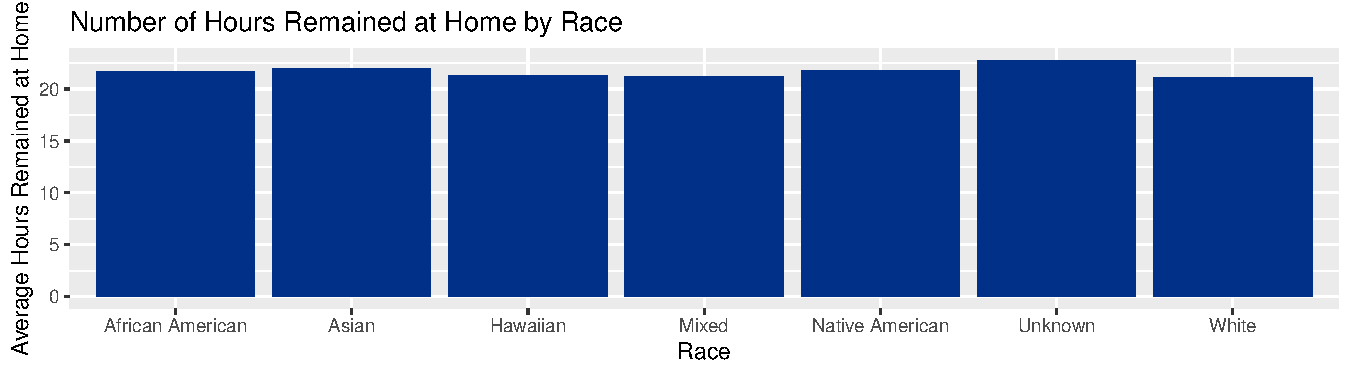
\includegraphics{finalreport_template_files/figure-latex/data-analysis-2.pdf}

\begin{Shaded}
\begin{Highlighting}[]
\FunctionTok{ggplot}\NormalTok{(}\AttributeTok{data=}\NormalTok{reasons\_for\_leaving, }\FunctionTok{aes}\NormalTok{(}\AttributeTok{x=}\NormalTok{reasons, }\AttributeTok{y=}\NormalTok{freq\_reasons)) }\SpecialCharTok{+}
  \FunctionTok{geom\_bar}\NormalTok{(}\AttributeTok{stat=}\StringTok{"identity"}\NormalTok{, }\AttributeTok{fill =} \StringTok{"\#003087"}\NormalTok{) }\SpecialCharTok{+}
  \FunctionTok{labs}\NormalTok{ (}
    \AttributeTok{y =} \StringTok{"Frequency"}\NormalTok{,}
    \AttributeTok{x =} \StringTok{"Reasons"}\NormalTok{,}
    \AttributeTok{title =} \StringTok{"Reasons for Leaving the House"}\NormalTok{,}
\NormalTok{    ) }
\end{Highlighting}
\end{Shaded}

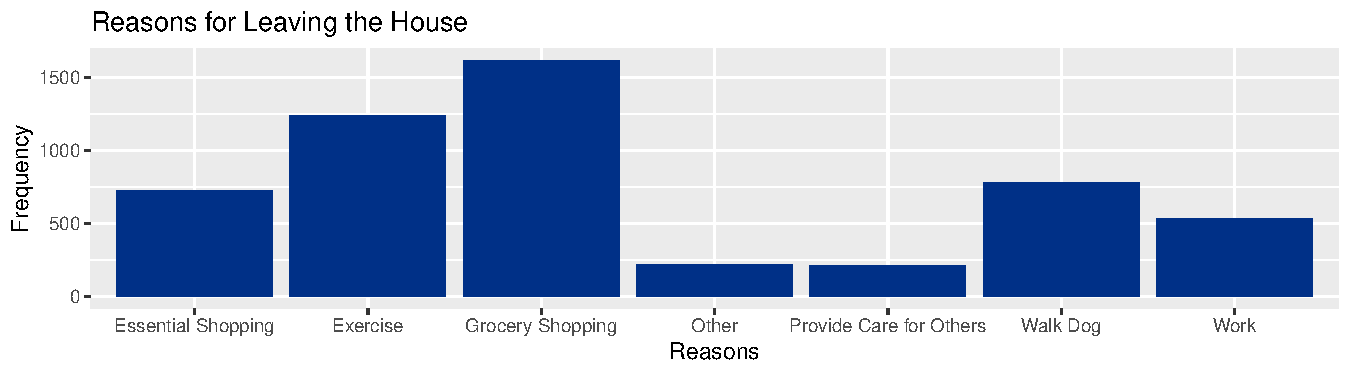
\includegraphics{finalreport_template_files/figure-latex/data-analysis-3.pdf}

\begin{Shaded}
\begin{Highlighting}[]
\CommentTok{\# preprocess data for t{-}tests}
\NormalTok{tidy\_data }\OtherTok{\textless{}{-}}\NormalTok{ tidy\_data }\SpecialCharTok{\%\textgreater{}\%}
  \FunctionTok{mutate}\NormalTok{(}\AttributeTok{asian =} \FunctionTok{ifelse}\NormalTok{(race }\SpecialCharTok{==} \StringTok{"Asian"}\NormalTok{, }\DecValTok{1}\NormalTok{, }\DecValTok{0}\NormalTok{)) }\SpecialCharTok{\%\textgreater{}\%}
  \FunctionTok{mutate}\NormalTok{(}\AttributeTok{white =} \FunctionTok{ifelse}\NormalTok{(race }\SpecialCharTok{==} \StringTok{"White"}\NormalTok{, }\DecValTok{1}\NormalTok{, }\DecValTok{0}\NormalTok{)) }\SpecialCharTok{\%\textgreater{}\%}
  \FunctionTok{mutate}\NormalTok{(}\AttributeTok{unknown =} \FunctionTok{ifelse}\NormalTok{(race }\SpecialCharTok{==} \StringTok{"Unknown"}\NormalTok{, }\DecValTok{1}\NormalTok{, }\DecValTok{0}\NormalTok{)) }\SpecialCharTok{\%\textgreater{}\%}
  \FunctionTok{mutate}\NormalTok{(}\AttributeTok{africanamerican =} \FunctionTok{ifelse}\NormalTok{(race }\SpecialCharTok{==} \StringTok{"African American"}\NormalTok{, }\DecValTok{1}\NormalTok{, }\DecValTok{0}\NormalTok{)) }\SpecialCharTok{\%\textgreater{}\%}
  \FunctionTok{mutate}\NormalTok{(}\AttributeTok{americanindian =} \FunctionTok{ifelse}\NormalTok{(race }\SpecialCharTok{==} \StringTok{"Native American"}\NormalTok{, }\DecValTok{1}\NormalTok{, }\DecValTok{0}\NormalTok{)) }\SpecialCharTok{\%\textgreater{}\%}
  \FunctionTok{mutate}\NormalTok{(}\AttributeTok{mixed =} \FunctionTok{ifelse}\NormalTok{(race }\SpecialCharTok{==} \StringTok{"Mixed"}\NormalTok{, }\DecValTok{1}\NormalTok{, }\DecValTok{0}\NormalTok{)) }\SpecialCharTok{\%\textgreater{}\%}
  \FunctionTok{mutate}\NormalTok{(}\AttributeTok{hawaiian =} \FunctionTok{ifelse}\NormalTok{(race }\SpecialCharTok{==} \StringTok{"Hawaiian"}\NormalTok{, }\DecValTok{1}\NormalTok{, }\DecValTok{0}\NormalTok{)) }\SpecialCharTok{\%\textgreater{}\%}
  \FunctionTok{mutate}\NormalTok{(}\AttributeTok{noschool =} \FunctionTok{ifelse}\NormalTok{(educ }\SpecialCharTok{==} \DecValTok{1}\NormalTok{, }\DecValTok{1}\NormalTok{, }\DecValTok{0}\NormalTok{)) }\SpecialCharTok{\%\textgreater{}\%}
  \FunctionTok{mutate}\NormalTok{(}\AttributeTok{g1\_8 =} \FunctionTok{ifelse}\NormalTok{(educ }\SpecialCharTok{==} \DecValTok{2}\NormalTok{, }\DecValTok{1}\NormalTok{, }\DecValTok{0}\NormalTok{)) }\SpecialCharTok{\%\textgreater{}\%}
  \FunctionTok{mutate}\NormalTok{(}\AttributeTok{g9\_11 =} \FunctionTok{ifelse}\NormalTok{(educ }\SpecialCharTok{==} \DecValTok{3}\NormalTok{, }\DecValTok{1}\NormalTok{, }\DecValTok{0}\NormalTok{)) }\SpecialCharTok{\%\textgreater{}\%}
  \FunctionTok{mutate}\NormalTok{(}\AttributeTok{g12 =} \FunctionTok{ifelse}\NormalTok{(educ }\SpecialCharTok{==} \DecValTok{4}\NormalTok{, }\DecValTok{1}\NormalTok{, }\DecValTok{0}\NormalTok{)) }\SpecialCharTok{\%\textgreater{}\%}
  \FunctionTok{mutate}\NormalTok{(}\AttributeTok{technical\_college =} \FunctionTok{ifelse}\NormalTok{(educ }\SpecialCharTok{==} \DecValTok{5}\NormalTok{, }\DecValTok{1}\NormalTok{, }\DecValTok{0}\NormalTok{)) }\SpecialCharTok{\%\textgreater{}\%}
  \FunctionTok{mutate}\NormalTok{(}\AttributeTok{four\_years\_college =} \FunctionTok{ifelse}\NormalTok{(educ }\SpecialCharTok{==} \DecValTok{6}\NormalTok{, }\DecValTok{1}\NormalTok{, }\DecValTok{0}\NormalTok{)) }\SpecialCharTok{\%\textgreater{}\%}
  \FunctionTok{mutate}\NormalTok{(}\AttributeTok{poorest =} \FunctionTok{ifelse}\NormalTok{(hhincome }\SpecialCharTok{==} \DecValTok{1}\NormalTok{, }\DecValTok{1}\NormalTok{, }\DecValTok{0}\NormalTok{)) }\SpecialCharTok{\%\textgreater{}\%}
  \FunctionTok{mutate}\NormalTok{(}\AttributeTok{richest =} \FunctionTok{ifelse}\NormalTok{(hhincome }\SpecialCharTok{==} \DecValTok{12}\NormalTok{, }\DecValTok{1}\NormalTok{, }\DecValTok{0}\NormalTok{))}
  
\CommentTok{\# t{-}test by EDUCATION insignificant p{-}value (do not reject null hypothesis)}
\CommentTok{\# t.test(tidy\_data$localsiphours\textasciitilde{}tidy\_data$noschool, var.equal=FALSE)}
\CommentTok{\# t.test(tidy\_data$localsiphours\textasciitilde{}tidy\_data$g1\_8, var.equal=FALSE)}
\FunctionTok{t.test}\NormalTok{(tidy\_data}\SpecialCharTok{$}\NormalTok{localsiphours}\SpecialCharTok{\textasciitilde{}}\NormalTok{tidy\_data}\SpecialCharTok{$}\NormalTok{g9\_11, }\AttributeTok{var.equal=}\ConstantTok{FALSE}\NormalTok{)}
\end{Highlighting}
\end{Shaded}

\begin{verbatim}
## 
##  Welch Two Sample t-test
## 
## data:  tidy_data$localsiphours by tidy_data$g9_11
## t = 0.92639, df = 1.0016, p-value = 0.5241
## alternative hypothesis: true difference in means between group 0 and group 1 is not equal to 0
## 95 percent confidence interval:
##  -123.2403  142.7021
## sample estimates:
## mean in group 0 mean in group 1 
##        21.23089        11.50000
\end{verbatim}

\begin{Shaded}
\begin{Highlighting}[]
\FunctionTok{t.test}\NormalTok{(tidy\_data}\SpecialCharTok{$}\NormalTok{localsiphours}\SpecialCharTok{\textasciitilde{}}\NormalTok{tidy\_data}\SpecialCharTok{$}\NormalTok{g12, }\AttributeTok{var.equal=}\ConstantTok{FALSE}\NormalTok{)}
\end{Highlighting}
\end{Shaded}

\begin{verbatim}
## 
##  Welch Two Sample t-test
## 
## data:  tidy_data$localsiphours by tidy_data$g12
## t = -0.73531, df = 44.873, p-value = 0.466
## alternative hypothesis: true difference in means between group 0 and group 1 is not equal to 0
## 95 percent confidence interval:
##  -2.185161  1.016422
## sample estimates:
## mean in group 0 mean in group 1 
##        21.20975        21.79412
\end{verbatim}

\begin{Shaded}
\begin{Highlighting}[]
\FunctionTok{t.test}\NormalTok{(tidy\_data}\SpecialCharTok{$}\NormalTok{localsiphours}\SpecialCharTok{\textasciitilde{}}\NormalTok{tidy\_data}\SpecialCharTok{$}\NormalTok{technical\_college, }\AttributeTok{var.equal=}\ConstantTok{FALSE}\NormalTok{)}
\end{Highlighting}
\end{Shaded}

\begin{verbatim}
## 
##  Welch Two Sample t-test
## 
## data:  tidy_data$localsiphours by tidy_data$technical_college
## t = 2.3857, df = 957.77, p-value = 0.01724
## alternative hypothesis: true difference in means between group 0 and group 1 is not equal to 0
## 95 percent confidence interval:
##  0.1994046 2.0485164
## sample estimates:
## mean in group 0 mean in group 1 
##        21.38056        20.25660
\end{verbatim}

\begin{Shaded}
\begin{Highlighting}[]
\FunctionTok{t.test}\NormalTok{(tidy\_data}\SpecialCharTok{$}\NormalTok{localsiphours}\SpecialCharTok{\textasciitilde{}}\NormalTok{tidy\_data}\SpecialCharTok{$}\NormalTok{four\_years\_college, }\AttributeTok{var.equal=}\ConstantTok{FALSE}\NormalTok{)}
\end{Highlighting}
\end{Shaded}

\begin{verbatim}
## 
##  Welch Two Sample t-test
## 
## data:  tidy_data$localsiphours by tidy_data$four_years_college
## t = -2.1467, df = 1198.5, p-value = 0.03202
## alternative hypothesis: true difference in means between group 0 and group 1 is not equal to 0
## 95 percent confidence interval:
##  -1.89997377 -0.08543864
## sample estimates:
## mean in group 0 mean in group 1 
##        20.38944        21.38215
\end{verbatim}

\begin{Shaded}
\begin{Highlighting}[]
\CommentTok{\# t{-}test by RACE insignificant p{-}value (do not reject null hypothesis)}
\FunctionTok{t.test}\NormalTok{(tidy\_data}\SpecialCharTok{$}\NormalTok{localsiphours}\SpecialCharTok{\textasciitilde{}}\NormalTok{tidy\_data}\SpecialCharTok{$}\NormalTok{asian, }\AttributeTok{var.equal=}\ConstantTok{FALSE}\NormalTok{)}
\end{Highlighting}
\end{Shaded}

\begin{verbatim}
## 
##  Welch Two Sample t-test
## 
## data:  tidy_data$localsiphours by tidy_data$asian
## t = -1.4506, df = 218.19, p-value = 0.1483
## alternative hypothesis: true difference in means between group 0 and group 1 is not equal to 0
## 95 percent confidence interval:
##  -1.7639892  0.2682241
## sample estimates:
## mean in group 0 mean in group 1 
##        21.18690        21.93478
\end{verbatim}

\begin{Shaded}
\begin{Highlighting}[]
\FunctionTok{t.test}\NormalTok{(tidy\_data}\SpecialCharTok{$}\NormalTok{localsiphours}\SpecialCharTok{\textasciitilde{}}\NormalTok{tidy\_data}\SpecialCharTok{$}\NormalTok{white, }\AttributeTok{var.equal=}\ConstantTok{FALSE}\NormalTok{)}
\end{Highlighting}
\end{Shaded}

\begin{verbatim}
## 
##  Welch Two Sample t-test
## 
## data:  tidy_data$localsiphours by tidy_data$white
## t = 1.5607, df = 1257.6, p-value = 0.1189
## alternative hypothesis: true difference in means between group 0 and group 1 is not equal to 0
## 95 percent confidence interval:
##  -0.1629826  1.4310749
## sample estimates:
## mean in group 0 mean in group 1 
##        21.78505        21.15100
\end{verbatim}

\begin{Shaded}
\begin{Highlighting}[]
\FunctionTok{t.test}\NormalTok{(tidy\_data}\SpecialCharTok{$}\NormalTok{localsiphours}\SpecialCharTok{\textasciitilde{}}\NormalTok{tidy\_data}\SpecialCharTok{$}\NormalTok{africanamerican, }\AttributeTok{var.equal=}\ConstantTok{FALSE}\NormalTok{)}
\end{Highlighting}
\end{Shaded}

\begin{verbatim}
## 
##  Welch Two Sample t-test
## 
## data:  tidy_data$localsiphours by tidy_data$africanamerican
## t = -0.8345, df = 59.915, p-value = 0.4073
## alternative hypothesis: true difference in means between group 0 and group 1 is not equal to 0
## 95 percent confidence interval:
##  -1.5669406  0.6444163
## sample estimates:
## mean in group 0 mean in group 1 
##        21.21616        21.67742
\end{verbatim}

\begin{Shaded}
\begin{Highlighting}[]
\FunctionTok{t.test}\NormalTok{(tidy\_data}\SpecialCharTok{$}\NormalTok{localsiphours}\SpecialCharTok{\textasciitilde{}}\NormalTok{tidy\_data}\SpecialCharTok{$}\NormalTok{americanindian, }\AttributeTok{var.equal=}\ConstantTok{FALSE}\NormalTok{)}
\end{Highlighting}
\end{Shaded}

\begin{verbatim}
## 
##  Welch Two Sample t-test
## 
## data:  tidy_data$localsiphours by tidy_data$americanindian
## t = -0.52001, df = 14.14, p-value = 0.6111
## alternative hypothesis: true difference in means between group 0 and group 1 is not equal to 0
## 95 percent confidence interval:
##  -2.812414  1.713952
## sample estimates:
## mean in group 0 mean in group 1 
##        21.22000        21.76923
\end{verbatim}

\begin{Shaded}
\begin{Highlighting}[]
\FunctionTok{t.test}\NormalTok{(tidy\_data}\SpecialCharTok{$}\NormalTok{localsiphours}\SpecialCharTok{\textasciitilde{}}\NormalTok{tidy\_data}\SpecialCharTok{$}\NormalTok{mixed, }\AttributeTok{var.equal=}\ConstantTok{FALSE}\NormalTok{)}
\end{Highlighting}
\end{Shaded}

\begin{verbatim}
## 
##  Welch Two Sample t-test
## 
## data:  tidy_data$localsiphours by tidy_data$mixed
## t = 0.091563, df = 98.419, p-value = 0.9272
## alternative hypothesis: true difference in means between group 0 and group 1 is not equal to 0
## 95 percent confidence interval:
##  -1.079356  1.183782
## sample estimates:
## mean in group 0 mean in group 1 
##        21.22529        21.17308
\end{verbatim}

\begin{Shaded}
\begin{Highlighting}[]
\FunctionTok{t.test}\NormalTok{(tidy\_data}\SpecialCharTok{$}\NormalTok{localsiphours}\SpecialCharTok{\textasciitilde{}}\NormalTok{tidy\_data}\SpecialCharTok{$}\NormalTok{hawaiian, }\AttributeTok{var.equal=}\ConstantTok{FALSE}\NormalTok{)}
\end{Highlighting}
\end{Shaded}

\begin{verbatim}
## 
##  Welch Two Sample t-test
## 
## data:  tidy_data$localsiphours by tidy_data$hawaiian
## t = -0.04088, df = 2.0492, p-value = 0.971
## alternative hypothesis: true difference in means between group 0 and group 1 is not equal to 0
## 95 percent confidence interval:
##  -11.39162  11.17227
## sample estimates:
## mean in group 0 mean in group 1 
##        21.22366        21.33333
\end{verbatim}

\begin{Shaded}
\begin{Highlighting}[]
\CommentTok{\# t{-}test by INCOME LEVEL}
\FunctionTok{t.test}\NormalTok{(tidy\_data}\SpecialCharTok{$}\NormalTok{localsiphours}\SpecialCharTok{\textasciitilde{}}\NormalTok{tidy\_data}\SpecialCharTok{$}\NormalTok{poorest, }\AttributeTok{var.equal=}\ConstantTok{FALSE}\NormalTok{)}
\end{Highlighting}
\end{Shaded}

\begin{verbatim}
## 
##  Welch Two Sample t-test
## 
## data:  tidy_data$localsiphours by tidy_data$poorest
## t = -0.30494, df = 44.42, p-value = 0.7618
## alternative hypothesis: true difference in means between group 0 and group 1 is not equal to 0
## 95 percent confidence interval:
##  -1.452853  1.070890
## sample estimates:
## mean in group 0 mean in group 1 
##        21.21643        21.40741
\end{verbatim}

\begin{Shaded}
\begin{Highlighting}[]
\FunctionTok{t.test}\NormalTok{(tidy\_data}\SpecialCharTok{$}\NormalTok{localsiphours}\SpecialCharTok{\textasciitilde{}}\NormalTok{tidy\_data}\SpecialCharTok{$}\NormalTok{richest, }\AttributeTok{var.equal=}\ConstantTok{FALSE}\NormalTok{)}
\end{Highlighting}
\end{Shaded}

\begin{verbatim}
## 
##  Welch Two Sample t-test
## 
## data:  tidy_data$localsiphours by tidy_data$richest
## t = 0.63165, df = 1381.7, p-value = 0.5277
## alternative hypothesis: true difference in means between group 0 and group 1 is not equal to 0
## 95 percent confidence interval:
##  -0.6866933  1.3389351
## sample estimates:
## mean in group 0 mean in group 1 
##        21.34941        21.02329
\end{verbatim}

\begin{Shaded}
\begin{Highlighting}[]
\CommentTok{\# t{-}test by RACE significant p{-}value (reject null hypothesis)}
\FunctionTok{t.test}\NormalTok{(tidy\_data}\SpecialCharTok{$}\NormalTok{localsiphours}\SpecialCharTok{\textasciitilde{}}\NormalTok{tidy\_data}\SpecialCharTok{$}\NormalTok{unknown, }\AttributeTok{var.equal=}\ConstantTok{FALSE}\NormalTok{)}
\end{Highlighting}
\end{Shaded}

\begin{verbatim}
## 
##  Welch Two Sample t-test
## 
## data:  tidy_data$localsiphours by tidy_data$unknown
## t = -4.2165, df = 158.94, p-value = 4.153e-05
## alternative hypothesis: true difference in means between group 0 and group 1 is not equal to 0
## 95 percent confidence interval:
##  -2.3175201 -0.8390017
## sample estimates:
## mean in group 0 mean in group 1 
##        21.20435        22.78261
\end{verbatim}

\begin{Shaded}
\begin{Highlighting}[]
\CommentTok{\# t{-}test by SEX significant p{-}value (reject null hypothesis)}
\FunctionTok{t.test}\NormalTok{(tidy\_data}\SpecialCharTok{$}\NormalTok{localsiphours}\SpecialCharTok{\textasciitilde{}}\NormalTok{tidy\_data}\SpecialCharTok{$}\NormalTok{sex, }\AttributeTok{var.equal=}\ConstantTok{FALSE}\NormalTok{)}
\end{Highlighting}
\end{Shaded}

\begin{verbatim}
## 
##  Welch Two Sample t-test
## 
## data:  tidy_data$localsiphours by tidy_data$sex
## t = -3.5035, df = 1809.3, p-value = 0.0004703
## alternative hypothesis: true difference in means between group 1 and group 2 is not equal to 0
## 95 percent confidence interval:
##  -2.5981696 -0.7332444
## sample estimates:
## mean in group 1 mean in group 2 
##        20.09075        21.75646
\end{verbatim}

\begin{Shaded}
\begin{Highlighting}[]
\CommentTok{\# ANOVA with UNKOWN}
\FunctionTok{summary}\NormalTok{(}\FunctionTok{aov}\NormalTok{(localsiphours}\SpecialCharTok{\textasciitilde{}}\NormalTok{race,}\AttributeTok{data=}\NormalTok{tidy\_data))}
\end{Highlighting}
\end{Shaded}

\begin{verbatim}
##               Df Sum Sq Mean Sq F value Pr(>F)
## race           6    122   20.26   0.125  0.993
## Residuals   1856 300760  162.05
\end{verbatim}

\begin{Shaded}
\begin{Highlighting}[]
\FunctionTok{summary}\NormalTok{(}\FunctionTok{aov}\NormalTok{(localsiphours}\SpecialCharTok{\textasciitilde{}}\NormalTok{state,}\AttributeTok{data=}\NormalTok{tidy\_data))}
\end{Highlighting}
\end{Shaded}

\begin{verbatim}
##               Df Sum Sq Mean Sq F value Pr(>F)
## state          1    198   198.1   1.216   0.27
## Residuals   1845 300564   162.9               
## 16 observations deleted due to missingness
\end{verbatim}

\begin{Shaded}
\begin{Highlighting}[]
\CommentTok{\# filter out unkonwn and observe results}
\NormalTok{tidy\_data\_without\_unknown }\OtherTok{\textless{}{-}}\NormalTok{ tidy\_data }\SpecialCharTok{\%\textgreater{}\%}
  \FunctionTok{filter}\NormalTok{(unknown }\SpecialCharTok{==}\DecValTok{0}\NormalTok{)}

\CommentTok{\# ANOVA test}
\FunctionTok{summary}\NormalTok{(}\FunctionTok{aov}\NormalTok{(localsiphours}\SpecialCharTok{\textasciitilde{}}\NormalTok{race,}\AttributeTok{data=}\NormalTok{tidy\_data\_without\_unknown))}
\end{Highlighting}
\end{Shaded}

\begin{verbatim}
##               Df Sum Sq Mean Sq F value Pr(>F)
## race           5     65   12.99   0.079  0.995
## Residuals   1834 300734  163.98
\end{verbatim}

\begin{Shaded}
\begin{Highlighting}[]
\FunctionTok{summary}\NormalTok{(}\FunctionTok{aov}\NormalTok{(localsiphours}\SpecialCharTok{\textasciitilde{}}\NormalTok{state,}\AttributeTok{data=}\NormalTok{tidy\_data\_without\_unknown))}
\end{Highlighting}
\end{Shaded}

\begin{verbatim}
##               Df Sum Sq Mean Sq F value Pr(>F)
## state          1    188   187.5   1.137  0.286
## Residuals   1822 300491   164.9               
## 16 observations deleted due to missingness
\end{verbatim}

\begin{Shaded}
\begin{Highlighting}[]
\CommentTok{\# 95\% confidence interval by race}
\NormalTok{dt }\OtherTok{\textless{}{-}}\NormalTok{ tidy\_data}\SpecialCharTok{\%\textgreater{}\%}
  \FunctionTok{group\_by}\NormalTok{(race)}\SpecialCharTok{\%\textgreater{}\%}
  \FunctionTok{filter}\NormalTok{(race }\SpecialCharTok{!=} \StringTok{"Hawaiian"}\NormalTok{)}\SpecialCharTok{\%\textgreater{}\%}
  \FunctionTok{summarise}\NormalTok{(}
    \AttributeTok{mean =} \FunctionTok{mean}\NormalTok{(localsiphours),}
    \AttributeTok{lci =} \FunctionTok{t.test}\NormalTok{(localsiphours, }\AttributeTok{conf.level =} \FloatTok{0.95}\NormalTok{)}\SpecialCharTok{$}\NormalTok{conf.int[}\DecValTok{1}\NormalTok{],}
    \AttributeTok{uci =} \FunctionTok{t.test}\NormalTok{(localsiphours, }\AttributeTok{conf.level =} \FloatTok{0.95}\NormalTok{)}\SpecialCharTok{$}\NormalTok{conf.int[}\DecValTok{2}\NormalTok{])}
\NormalTok{dt}
\end{Highlighting}
\end{Shaded}

\begin{verbatim}
## # A tibble: 6 x 4
##   race              mean   lci   uci
##   <chr>            <dbl> <dbl> <dbl>
## 1 African American  21.7  20.7  22.6
## 2 Asian             21.9  21.1  22.8
## 3 Mixed             21.2  20.2  22.1
## 4 Native American   21.8  19.6  24.0
## 5 Unknown           22.8  22.3  23.3
## 6 White             21.2  20.5  21.8
\end{verbatim}

\begin{Shaded}
\begin{Highlighting}[]
\NormalTok{pl2 }\OtherTok{\textless{}{-}} \FunctionTok{ggplot}\NormalTok{(}\AttributeTok{data =}\NormalTok{ dt)}
\NormalTok{pl2 }\OtherTok{\textless{}{-}}\NormalTok{ pl2 }\SpecialCharTok{+} \FunctionTok{geom\_point}\NormalTok{(}\FunctionTok{aes}\NormalTok{(}\AttributeTok{x=}\NormalTok{race, }\AttributeTok{y=}\NormalTok{mean), }\AttributeTok{color=} \StringTok{"red"}\NormalTok{)}
\NormalTok{pl2 }\OtherTok{\textless{}{-}}\NormalTok{ pl2 }\SpecialCharTok{+} \FunctionTok{geom\_errorbar}\NormalTok{(}\FunctionTok{aes}\NormalTok{(}\AttributeTok{x=}\NormalTok{race, }\AttributeTok{ymin=}\NormalTok{lci, }\AttributeTok{ymax=}\NormalTok{ uci), }\AttributeTok{width =} \FloatTok{0.4}\NormalTok{, }\AttributeTok{color =}\StringTok{"red"}\NormalTok{, }\AttributeTok{size =} \DecValTok{1}\NormalTok{)}
\NormalTok{pl2 }\OtherTok{\textless{}{-}}\NormalTok{ pl2 }\SpecialCharTok{+} \FunctionTok{geom\_text}\NormalTok{(}\FunctionTok{aes}\NormalTok{(}\AttributeTok{x=}\NormalTok{race, }\AttributeTok{y=}\NormalTok{lci, }\AttributeTok{label =} \FunctionTok{round}\NormalTok{(lci,}\DecValTok{1}\NormalTok{)), }\AttributeTok{size=} \DecValTok{2}\NormalTok{, }\AttributeTok{vjust =} \DecValTok{1}\NormalTok{)}
\NormalTok{pl2 }\OtherTok{\textless{}{-}}\NormalTok{ pl2 }\SpecialCharTok{+} \FunctionTok{geom\_text}\NormalTok{(}\FunctionTok{aes}\NormalTok{(}\AttributeTok{x=}\NormalTok{race, }\AttributeTok{y=}\NormalTok{uci, }\AttributeTok{label =} \FunctionTok{round}\NormalTok{(uci,}\DecValTok{1}\NormalTok{)), }\AttributeTok{size=} \DecValTok{2}\NormalTok{, }\AttributeTok{vjust =} \SpecialCharTok{{-}}\DecValTok{1}\NormalTok{)}
\NormalTok{pl2 }\OtherTok{\textless{}{-}}\NormalTok{ pl2 }\SpecialCharTok{+} \FunctionTok{theme\_classic}\NormalTok{()}
\NormalTok{pl2 }\OtherTok{\textless{}{-}}\NormalTok{ pl2 }\SpecialCharTok{+} \FunctionTok{labs}\NormalTok{(}\AttributeTok{title =} \StringTok{"Mean Hours Spent at Home with 95\% Confidence Intervals"}\NormalTok{)}
\NormalTok{pl2 }\OtherTok{\textless{}{-}}\NormalTok{ pl2 }\SpecialCharTok{+} \FunctionTok{labs}\NormalTok{(}\AttributeTok{x=} \StringTok{"Race"}\NormalTok{, }\AttributeTok{y =} \StringTok{"Mean Hours Spent Home"}\NormalTok{)}
\NormalTok{pl2}
\end{Highlighting}
\end{Shaded}

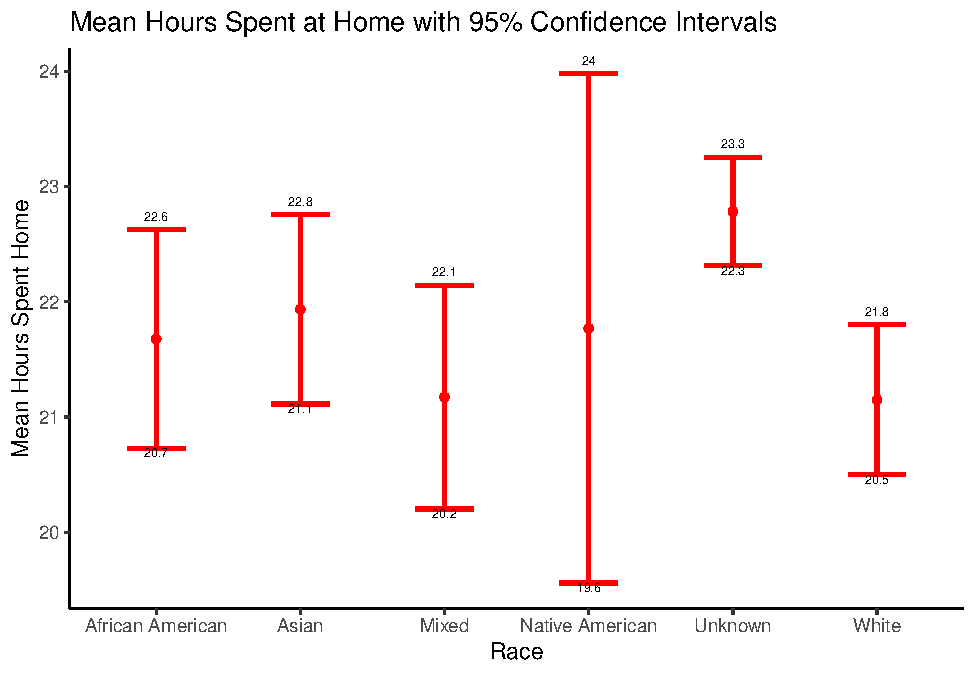
\includegraphics{finalreport_template_files/figure-latex/confidence_interval_plots-1.pdf}

\begin{Shaded}
\begin{Highlighting}[]
\CommentTok{\# 95\% confidence interval by education}
\NormalTok{tidy\_data}\SpecialCharTok{$}\NormalTok{educ[tidy\_data}\SpecialCharTok{$}\NormalTok{educ }\SpecialCharTok{==} \DecValTok{1}\NormalTok{] }\OtherTok{\textless{}{-}} \StringTok{"No School"}
\NormalTok{tidy\_data}\SpecialCharTok{$}\NormalTok{educ[tidy\_data}\SpecialCharTok{$}\NormalTok{educ }\SpecialCharTok{==} \DecValTok{2}\NormalTok{] }\OtherTok{\textless{}{-}} \StringTok{"G1{-}8"}
\NormalTok{tidy\_data}\SpecialCharTok{$}\NormalTok{educ[tidy\_data}\SpecialCharTok{$}\NormalTok{educ }\SpecialCharTok{==} \DecValTok{3}\NormalTok{] }\OtherTok{\textless{}{-}} \StringTok{"G9{-}12"}
\NormalTok{tidy\_data}\SpecialCharTok{$}\NormalTok{educ[tidy\_data}\SpecialCharTok{$}\NormalTok{educ }\SpecialCharTok{==} \DecValTok{4}\NormalTok{] }\OtherTok{\textless{}{-}} \StringTok{"GED"}
\NormalTok{tidy\_data}\SpecialCharTok{$}\NormalTok{educ[tidy\_data}\SpecialCharTok{$}\NormalTok{educ }\SpecialCharTok{==} \DecValTok{5}\NormalTok{] }\OtherTok{\textless{}{-}} \StringTok{"Some College"}
\NormalTok{tidy\_data}\SpecialCharTok{$}\NormalTok{educ[tidy\_data}\SpecialCharTok{$}\NormalTok{educ }\SpecialCharTok{==} \DecValTok{6}\NormalTok{] }\OtherTok{\textless{}{-}} \StringTok{"4 Years College"}
\NormalTok{tidy\_data}\SpecialCharTok{$}\NormalTok{educ[tidy\_data}\SpecialCharTok{$}\NormalTok{educ }\SpecialCharTok{==} \DecValTok{7}\NormalTok{] }\OtherTok{\textless{}{-}} \StringTok{"Not Sure"}
\NormalTok{tidy\_data}\SpecialCharTok{$}\NormalTok{educ[}\FunctionTok{is.na}\NormalTok{(tidy\_data}\SpecialCharTok{$}\NormalTok{educ)] }\OtherTok{\textless{}{-}} \StringTok{"Not Sure"}

\NormalTok{dt }\OtherTok{\textless{}{-}}\NormalTok{ tidy\_data}\SpecialCharTok{\%\textgreater{}\%}
  \FunctionTok{group\_by}\NormalTok{(educ)}\SpecialCharTok{\%\textgreater{}\%}
  \FunctionTok{filter}\NormalTok{(educ }\SpecialCharTok{!=} \StringTok{"G9{-}12"}\NormalTok{)}\SpecialCharTok{\%\textgreater{}\%}
  \FunctionTok{summarise}\NormalTok{(}
    \AttributeTok{mean =} \FunctionTok{mean}\NormalTok{(localsiphours),}
    \AttributeTok{lci =} \FunctionTok{t.test}\NormalTok{(localsiphours, }\AttributeTok{conf.level =} \FloatTok{0.95}\NormalTok{)}\SpecialCharTok{$}\NormalTok{conf.int[}\DecValTok{1}\NormalTok{],}
    \AttributeTok{uci =} \FunctionTok{t.test}\NormalTok{(localsiphours, }\AttributeTok{conf.level =} \FloatTok{0.95}\NormalTok{)}\SpecialCharTok{$}\NormalTok{conf.int[}\DecValTok{2}\NormalTok{])}
\NormalTok{dt}
\end{Highlighting}
\end{Shaded}

\begin{verbatim}
## # A tibble: 4 x 4
##   educ             mean   lci   uci
##   <chr>           <dbl> <dbl> <dbl>
## 1 4 Years College  21.4  20.7  22.1
## 2 GED              21.8  20.3  23.3
## 3 Not Sure         23.2  21.8  24.6
## 4 Some College     20.3  19.6  20.9
\end{verbatim}

\begin{Shaded}
\begin{Highlighting}[]
\NormalTok{pl2 }\OtherTok{\textless{}{-}} \FunctionTok{ggplot}\NormalTok{(}\AttributeTok{data =}\NormalTok{ dt)}
\NormalTok{pl2 }\OtherTok{\textless{}{-}}\NormalTok{ pl2 }\SpecialCharTok{+} \FunctionTok{geom\_point}\NormalTok{(}\FunctionTok{aes}\NormalTok{(}\AttributeTok{x=}\NormalTok{educ, }\AttributeTok{y=}\NormalTok{mean), }\AttributeTok{color=} \StringTok{"red"}\NormalTok{)}
\NormalTok{pl2 }\OtherTok{\textless{}{-}}\NormalTok{ pl2 }\SpecialCharTok{+} \FunctionTok{geom\_errorbar}\NormalTok{(}\FunctionTok{aes}\NormalTok{(}\AttributeTok{x=}\NormalTok{educ, }\AttributeTok{ymin=}\NormalTok{lci, }\AttributeTok{ymax=}\NormalTok{ uci), }\AttributeTok{width =} \FloatTok{0.4}\NormalTok{, }\AttributeTok{color =}\StringTok{"red"}\NormalTok{, }\AttributeTok{size =} \DecValTok{1}\NormalTok{)}
\NormalTok{pl2 }\OtherTok{\textless{}{-}}\NormalTok{ pl2 }\SpecialCharTok{+} \FunctionTok{geom\_text}\NormalTok{(}\FunctionTok{aes}\NormalTok{(}\AttributeTok{x=}\NormalTok{educ, }\AttributeTok{y=}\NormalTok{lci, }\AttributeTok{label =} \FunctionTok{round}\NormalTok{(lci,}\DecValTok{1}\NormalTok{)), }\AttributeTok{size=} \DecValTok{2}\NormalTok{, }\AttributeTok{vjust =} \DecValTok{1}\NormalTok{)}
\NormalTok{pl2 }\OtherTok{\textless{}{-}}\NormalTok{ pl2 }\SpecialCharTok{+} \FunctionTok{geom\_text}\NormalTok{(}\FunctionTok{aes}\NormalTok{(}\AttributeTok{x=}\NormalTok{educ, }\AttributeTok{y=}\NormalTok{uci, }\AttributeTok{label =} \FunctionTok{round}\NormalTok{(uci,}\DecValTok{1}\NormalTok{)), }\AttributeTok{size=} \DecValTok{2}\NormalTok{, }\AttributeTok{vjust =} \SpecialCharTok{{-}}\DecValTok{1}\NormalTok{)}
\NormalTok{pl2 }\OtherTok{\textless{}{-}}\NormalTok{ pl2 }\SpecialCharTok{+} \FunctionTok{theme\_classic}\NormalTok{()}
\NormalTok{pl2 }\OtherTok{\textless{}{-}}\NormalTok{ pl2 }\SpecialCharTok{+} \FunctionTok{labs}\NormalTok{(}\AttributeTok{title =} \StringTok{"Mean Hours Spent at Home with 95\% Confidence Intervals"}\NormalTok{)}
\NormalTok{pl2 }\OtherTok{\textless{}{-}}\NormalTok{ pl2 }\SpecialCharTok{+} \FunctionTok{labs}\NormalTok{(}\AttributeTok{x=} \StringTok{"Education Level"}\NormalTok{, }\AttributeTok{y =} \StringTok{"Mean Hours Spent Home"}\NormalTok{)}
\NormalTok{pl2}
\end{Highlighting}
\end{Shaded}

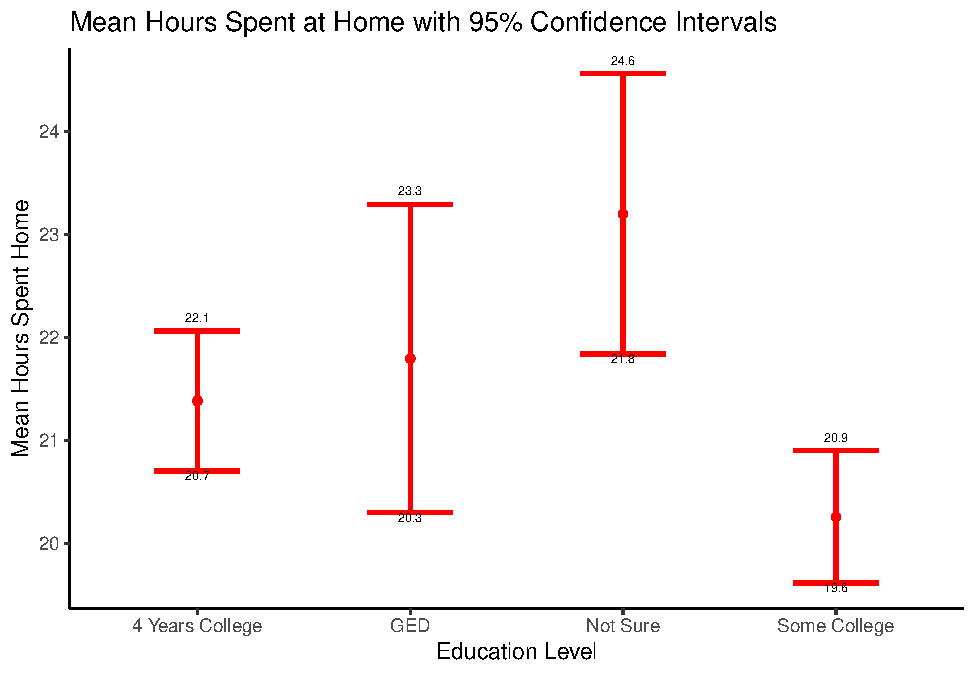
\includegraphics{finalreport_template_files/figure-latex/confidence_interval_plots-2.pdf}

\begin{Shaded}
\begin{Highlighting}[]
\CommentTok{\# 95\% confidence interval by income level}
\NormalTok{dt }\OtherTok{\textless{}{-}}\NormalTok{ tidy\_data}\SpecialCharTok{\%\textgreater{}\%}
  \FunctionTok{group\_by}\NormalTok{(hhincome)}\SpecialCharTok{\%\textgreater{}\%}
  \FunctionTok{filter}\NormalTok{(}\FunctionTok{is.na}\NormalTok{(hhincome) }\SpecialCharTok{==} \ConstantTok{FALSE}\NormalTok{)}\SpecialCharTok{\%\textgreater{}\%}
  \FunctionTok{summarise}\NormalTok{(}
    \AttributeTok{mean =} \FunctionTok{mean}\NormalTok{(localsiphours),}
    \AttributeTok{lci =} \FunctionTok{t.test}\NormalTok{(localsiphours, }\AttributeTok{conf.level =} \FloatTok{0.95}\NormalTok{)}\SpecialCharTok{$}\NormalTok{conf.int[}\DecValTok{1}\NormalTok{],}
    \AttributeTok{uci =} \FunctionTok{t.test}\NormalTok{(localsiphours, }\AttributeTok{conf.level =} \FloatTok{0.95}\NormalTok{)}\SpecialCharTok{$}\NormalTok{conf.int[}\DecValTok{2}\NormalTok{])}
\NormalTok{dt}
\end{Highlighting}
\end{Shaded}

\begin{verbatim}
## # A tibble: 12 x 4
##    hhincome  mean   lci   uci
##       <int> <dbl> <dbl> <dbl>
##  1        1  21.4  20.3  22.5
##  2        2  20.7  18.8  22.6
##  3        3  21.7  20.7  22.7
##  4        4  21.5  20.5  22.5
##  5        5  21.1  19.6  22.6
##  6        6  20.8  19.6  22.0
##  7        7  21.2  20.3  22.2
##  8        8  21.0  20.1  21.9
##  9        9  20.6  19.4  21.7
## 10       10  20.9  20.0  21.7
## 11       11  21.8  19.6  24.0
## 12       12  21.0  20.7  21.4
\end{verbatim}

\begin{Shaded}
\begin{Highlighting}[]
\NormalTok{pl2 }\OtherTok{\textless{}{-}} \FunctionTok{ggplot}\NormalTok{(}\AttributeTok{data =}\NormalTok{ dt)}
\NormalTok{pl2 }\OtherTok{\textless{}{-}}\NormalTok{ pl2 }\SpecialCharTok{+} \FunctionTok{geom\_point}\NormalTok{(}\FunctionTok{aes}\NormalTok{(}\AttributeTok{x=}\FunctionTok{as.factor}\NormalTok{(hhincome), }\AttributeTok{y=}\NormalTok{mean, }\AttributeTok{fill =} \FunctionTok{as.factor}\NormalTok{(hhincome)), }\AttributeTok{color=} \StringTok{"red"}\NormalTok{)}
\NormalTok{pl2 }\OtherTok{\textless{}{-}}\NormalTok{ pl2 }\SpecialCharTok{+} \FunctionTok{geom\_errorbar}\NormalTok{(}\FunctionTok{aes}\NormalTok{(}\AttributeTok{x=}\NormalTok{hhincome, }\AttributeTok{ymin=}\NormalTok{lci, }\AttributeTok{ymax=}\NormalTok{ uci), }\AttributeTok{width =} \FloatTok{0.4}\NormalTok{, }\AttributeTok{color =}\StringTok{"red"}\NormalTok{, }\AttributeTok{size =} \DecValTok{1}\NormalTok{)}
\NormalTok{pl2 }\OtherTok{\textless{}{-}}\NormalTok{ pl2 }\SpecialCharTok{+} \FunctionTok{geom\_text}\NormalTok{(}\FunctionTok{aes}\NormalTok{(}\AttributeTok{x=}\NormalTok{hhincome, }\AttributeTok{y=}\NormalTok{lci, }\AttributeTok{label =} \FunctionTok{round}\NormalTok{(lci,}\DecValTok{1}\NormalTok{)), }\AttributeTok{size=} \DecValTok{2}\NormalTok{, }\AttributeTok{vjust =} \DecValTok{1}\NormalTok{)}
\NormalTok{pl2 }\OtherTok{\textless{}{-}}\NormalTok{ pl2 }\SpecialCharTok{+} \FunctionTok{geom\_text}\NormalTok{(}\FunctionTok{aes}\NormalTok{(}\AttributeTok{x=}\NormalTok{hhincome, }\AttributeTok{y=}\NormalTok{uci, }\AttributeTok{label =} \FunctionTok{round}\NormalTok{(uci,}\DecValTok{1}\NormalTok{)), }\AttributeTok{size=} \DecValTok{2}\NormalTok{, }\AttributeTok{vjust =} \SpecialCharTok{{-}}\DecValTok{1}\NormalTok{)}
\NormalTok{pl2 }\OtherTok{\textless{}{-}}\NormalTok{ pl2 }\SpecialCharTok{+} \FunctionTok{theme\_classic}\NormalTok{()}
\NormalTok{pl2 }\OtherTok{\textless{}{-}}\NormalTok{ pl2 }\SpecialCharTok{+} \FunctionTok{labs}\NormalTok{(}\AttributeTok{title =} \StringTok{"Mean Hours Spent at Home with 95\% Confidence Intervals"}\NormalTok{)}
\NormalTok{pl2 }\OtherTok{\textless{}{-}}\NormalTok{ pl2 }\SpecialCharTok{+} \FunctionTok{labs}\NormalTok{(}\AttributeTok{x=} \StringTok{"Income Level"}\NormalTok{, }\AttributeTok{y =} \StringTok{"Mean Hours Spent Home"}\NormalTok{, }\AttributeTok{fill =} \StringTok{"okay"}\NormalTok{)}
\NormalTok{pl2 }\OtherTok{\textless{}{-}}\NormalTok{ pl2 }\SpecialCharTok{+} \FunctionTok{scale\_fill\_discrete}\NormalTok{(}\AttributeTok{name =} \StringTok{"Income Levels"}\NormalTok{, }\AttributeTok{labels =} \FunctionTok{c}\NormalTok{(}\StringTok{"1 {-} less than $9,999"}\NormalTok{, }\StringTok{"2 {-} $10,000 to $19,999"}\NormalTok{, }\StringTok{"3 {-} $20,000 to $29,999"}\NormalTok{,}\StringTok{"4 {-} $30,000 to $39,999"}\NormalTok{, }\StringTok{"5 {-} $40,000 to $49,999"}\NormalTok{, }\StringTok{"6 {-} $50,000 to $59,999"}\NormalTok{,}\StringTok{"7 {-} $60,000 to $69,999"}\NormalTok{, }\StringTok{"8 {-} $70,000 to $79,999"}\NormalTok{, }\StringTok{"9 {-} $80,000 to $89,999"}\NormalTok{,}\StringTok{"10 {-} $90,000 to $99,999"}\NormalTok{, }\StringTok{"11 {-} $100,000 to $150,000"}\NormalTok{, }\StringTok{"12 {-} over $150,000"}\NormalTok{))}
\NormalTok{pl2}
\end{Highlighting}
\end{Shaded}

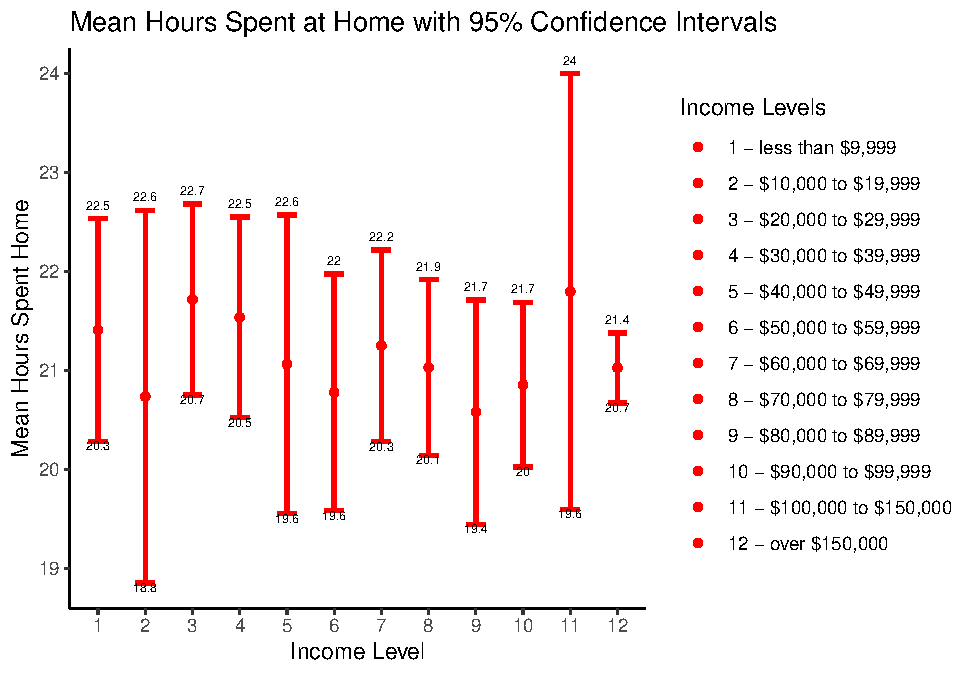
\includegraphics{finalreport_template_files/figure-latex/confidence_interval_plots-3.pdf}

\begin{Shaded}
\begin{Highlighting}[]
\CommentTok{\# fit logistic regression model with Education}
\NormalTok{localsiphours\_fit\_education }\OtherTok{\textless{}{-}} \FunctionTok{linear\_reg}\NormalTok{() }\SpecialCharTok{\%\textgreater{}\%}
  \FunctionTok{set\_engine}\NormalTok{(}\StringTok{"lm"}\NormalTok{) }\SpecialCharTok{\%\textgreater{}\%}
  \FunctionTok{fit}\NormalTok{(localsiphours }\SpecialCharTok{\textasciitilde{}}\NormalTok{ g9\_11 }\SpecialCharTok{+}\NormalTok{ technical\_college }\SpecialCharTok{+}\NormalTok{ four\_years\_college, }\AttributeTok{data =}\NormalTok{ tidy\_data)}

\CommentTok{\# fit logistic regression model with UNKNOWN}
\NormalTok{localsiphours\_fit }\OtherTok{\textless{}{-}} \FunctionTok{linear\_reg}\NormalTok{() }\SpecialCharTok{\%\textgreater{}\%}
  \FunctionTok{set\_engine}\NormalTok{(}\StringTok{"lm"}\NormalTok{) }\SpecialCharTok{\%\textgreater{}\%}
  \FunctionTok{fit}\NormalTok{(localsiphours }\SpecialCharTok{\textasciitilde{}}\NormalTok{ asian }\SpecialCharTok{+}\NormalTok{ white }\SpecialCharTok{+}\NormalTok{ africanamerican }\SpecialCharTok{+}\NormalTok{ americanindian }\SpecialCharTok{+}\NormalTok{ mixed }\SpecialCharTok{+}\NormalTok{ hawaiian, }\AttributeTok{data =}\NormalTok{ tidy\_data)}

\CommentTok{\#fit logistic regression model without UNKNOWN}
\NormalTok{localsiphours\_fit\_without\_unknown }\OtherTok{\textless{}{-}} \FunctionTok{linear\_reg}\NormalTok{() }\SpecialCharTok{\%\textgreater{}\%}
  \FunctionTok{set\_engine}\NormalTok{(}\StringTok{"lm"}\NormalTok{) }\SpecialCharTok{\%\textgreater{}\%}
  \FunctionTok{fit}\NormalTok{(localsiphours }\SpecialCharTok{\textasciitilde{}}\NormalTok{ asian }\SpecialCharTok{+}\NormalTok{ white }\SpecialCharTok{+}\NormalTok{ africanamerican }\SpecialCharTok{+}\NormalTok{ americanindian }\SpecialCharTok{+}\NormalTok{ mixed }\SpecialCharTok{+}\NormalTok{ hawaiian, }\AttributeTok{data =}\NormalTok{ tidy\_data\_without\_unknown)}

\CommentTok{\#fit logistic regression model without Association Terms}
\NormalTok{localsiphours\_fit\_without\_unknown\_association }\OtherTok{\textless{}{-}} \FunctionTok{linear\_reg}\NormalTok{() }\SpecialCharTok{\%\textgreater{}\%}
  \FunctionTok{set\_engine}\NormalTok{(}\StringTok{"lm"}\NormalTok{) }\SpecialCharTok{\%\textgreater{}\%}
  \FunctionTok{fit}\NormalTok{(localsiphours }\SpecialCharTok{\textasciitilde{}}\NormalTok{ asian }\SpecialCharTok{+}\NormalTok{ white }\SpecialCharTok{+}\NormalTok{ unknown }\SpecialCharTok{+}\NormalTok{ africanamerican }\SpecialCharTok{+}\NormalTok{ americanindian }\SpecialCharTok{+}\NormalTok{ mixed }\SpecialCharTok{+}\NormalTok{ hawaiian, }\AttributeTok{data =}\NormalTok{ tidy\_data)}

\FunctionTok{tidy}\NormalTok{(localsiphours\_fit, }\AttributeTok{conf.int=}\ConstantTok{TRUE}\NormalTok{, }\AttributeTok{exponentiate =} \ConstantTok{TRUE}\NormalTok{)}
\end{Highlighting}
\end{Shaded}

\begin{verbatim}
## # A tibble: 7 x 7
##   term            estimate std.error statistic  p.value conf.low conf.high
##   <chr>              <dbl>     <dbl>     <dbl>    <dbl>    <dbl>     <dbl>
## 1 (Intercept)       22.8        2.65     8.58  1.92e-17    17.6      28.0 
## 2 asian             -0.848      2.97    -0.286 7.75e- 1    -6.67      4.97
## 3 white             -1.63       2.67    -0.610 5.42e- 1    -6.87      3.61
## 4 africanamerican   -1.11       3.50    -0.315 7.52e- 1    -7.98      5.77
## 5 americanindian    -1.01       4.42    -0.229 8.19e- 1    -9.68      7.65
## 6 mixed             -1.61       3.19    -0.505 6.14e- 1    -7.86      4.64
## 7 hawaiian          -1.45       7.81    -0.185 8.53e- 1   -16.8      13.9
\end{verbatim}

\begin{Shaded}
\begin{Highlighting}[]
\FunctionTok{tidy}\NormalTok{(localsiphours\_fit\_without\_unknown, }\AttributeTok{conf.int=}\ConstantTok{TRUE}\NormalTok{, }\AttributeTok{exponentiate =} \ConstantTok{TRUE}\NormalTok{)}
\end{Highlighting}
\end{Shaded}

\begin{verbatim}
## # A tibble: 7 x 7
##   term            estimate std.error statistic  p.value conf.low conf.high
##   <chr>              <dbl>     <dbl>     <dbl>    <dbl>    <dbl>     <dbl>
## 1 (Intercept)       21.3        7.39    2.89    0.00395     6.83      35.8
## 2 asian              0.601      7.51    0.0801  0.936     -14.1       15.3
## 3 white             -0.182      7.40   -0.0246  0.980     -14.7       14.3
## 4 africanamerican    0.344      7.74    0.0444  0.965     -14.8       15.5
## 5 americanindian     0.436      8.20    0.0531  0.958     -15.7       16.5
## 6 mixed             -0.160      7.60   -0.0211  0.983     -15.1       14.8
## 7 hawaiian          NA         NA      NA      NA          NA         NA
\end{verbatim}

\begin{Shaded}
\begin{Highlighting}[]
\FunctionTok{tidy}\NormalTok{(localsiphours\_fit\_education, }\AttributeTok{conf.int=}\ConstantTok{TRUE}\NormalTok{, }\AttributeTok{exponentiate =} \ConstantTok{TRUE}\NormalTok{)}
\end{Highlighting}
\end{Shaded}

\begin{verbatim}
## # A tibble: 4 x 7
##   term               estimate std.error statistic  p.value conf.low conf.high
##   <chr>                 <dbl>     <dbl>     <dbl>    <dbl>    <dbl>     <dbl>
## 1 (Intercept)          21.9        2.12    10.3   2.81e-24    17.7      26.0 
## 2 g9_11               -10.4        9.24    -1.12  2.62e- 1   -28.5       7.76
## 3 technical_college    -1.60       2.26    -0.710 4.78e- 1    -6.04      2.83
## 4 four_years_college   -0.479      2.14    -0.223 8.23e- 1    -4.69      3.73
\end{verbatim}

\begin{Shaded}
\begin{Highlighting}[]
\FunctionTok{tidy}\NormalTok{(localsiphours\_fit\_without\_unknown\_association, }\AttributeTok{conf.int=}\ConstantTok{TRUE}\NormalTok{, }\AttributeTok{exponentiate =} \ConstantTok{TRUE}\NormalTok{)}
\end{Highlighting}
\end{Shaded}

\begin{verbatim}
## # A tibble: 8 x 7
##   term            estimate std.error statistic  p.value conf.low conf.high
##   <chr>              <dbl>     <dbl>     <dbl>    <dbl>    <dbl>     <dbl>
## 1 (Intercept)       21.3        7.35    2.90    0.00374     6.92      35.7
## 2 asian              0.601      7.47    0.0805  0.936     -14.0       15.2
## 3 white             -0.182      7.36   -0.0248  0.980     -14.6       14.2
## 4 unknown            1.45       7.81    0.185   0.853     -13.9       16.8
## 5 africanamerican    0.344      7.70    0.0447  0.964     -14.8       15.4
## 6 americanindian     0.436      8.15    0.0535  0.957     -15.6       16.4
## 7 mixed             -0.160      7.56   -0.0212  0.983     -15.0       14.7
## 8 hawaiian          NA         NA      NA      NA          NA         NA
\end{verbatim}

Conclusion

Limitations The sample over-represented Hispanic non-white individuals
while under-representing other races such as Black and Asian people.
Thus, our results may be skewed due to having small sample sizes for
certain demographics.

\end{document}
